% vim: set textwidth=120:

% Example CV based on the 1.5-column-cv template. Main features:
% * uses the Roboto font family and IcoMoon icon set;
% * doesn't use colours, different font weights are used instead for styling;
% * because the CV fits on one page, header and footer is empty, since there isn't much useful info to put there;
% * includes a photo.
\documentclass[a4paper,hidelinks,10pt]{article}


% package imports
% ---------------

\usepackage[british]{babel} % for correct language and hyphenation and stuff
\usepackage{calc}           % for easier length calculations (infix notation)
\usepackage{enumitem}       % for configuring list environments
\usepackage{fancyhdr}       % for setting header and footer
\usepackage{fontspec}       % for fonts
\usepackage{geometry}       % for setting margins (\newgeometry)
\usepackage{graphicx}       % for pictures
\usepackage{microtype}      % for microtypography stuff
\usepackage{xcolor}         % for colours
%\usepackage{hyperref}		% for links
\usepackage[hidelinks]{hyperref}


% margin and column widths
% ------------------------

% margins
\newgeometry{left=15mm,right=15mm,top=15mm,bottom=15mm}

% width of the gap between left and right column
\newlength{\cvcolumngapwidth}
\setlength{\cvcolumngapwidth}{3.5mm}

% left column width
\newlength{\cvleftcolumnwidth}
\setlength{\cvleftcolumnwidth}{44.5mm}

% right column width
\newlength{\cvrightcolumnwidth}
\setlength{\cvrightcolumnwidth}{\textwidth-\cvleftcolumnwidth-\cvcolumngapwidth}

% set paragraph indentation to 0, because it screws up the whole layout otherwise
\setlength{\parindent}{0mm}


% style definitions
% -----------------
% style categories explanation:
% * \cvnameXXX is used for the name;
% * \cvsectionXXX is used for section names (left column, accompanied by a horizontal rule);
% * \cvtitleXXX is used for job/education titles (right column);
% * \cvdurationXXX is used for job/education durations (left column);
% * \cvheadingXXX is used for headings (left column);
% * \cvmainXXX (and \setmainfont) is used for main text;
% * \cvruleXXX is used for the horizontal rules denoting sections.

% font families
\defaultfontfeatures{Ligatures=TeX} % reportedly a good idea, see https://tex.stackexchange.com/a/37251

\newfontfamily{\cvnamefont}{Roboto Medium}
\newfontfamily{\cvsectionfont}{Roboto Medium}
\newfontfamily{\cvtitlefont}{Roboto Regular}
\newfontfamily{\cvdurationfont}{Roboto Light Italic}
\newfontfamily{\cvheadingfont}{Roboto Regular}
\setmainfont{Roboto Light}

% colours
\definecolor{cvnamecolor}{HTML}{000000}
\definecolor{cvsectioncolor}{HTML}{000000}
\definecolor{cvtitlecolor}{HTML}{000000}
\definecolor{cvdurationcolor}{HTML}{000000}
\definecolor{cvheadingcolor}{HTML}{000000}
\definecolor{cvmaincolor}{HTML}{000000}
\definecolor{cvrulecolor}{HTML}{000000}

\color{cvmaincolor}

% styles
\newcommand{\cvnamestyle}[1]{{\Large\cvnamefont\textcolor{cvnamecolor}{#1}}}
\newcommand{\cvsectionstyle}[1]{{\normalsize\cvsectionfont\textcolor{cvsectioncolor}{#1}}}
\newcommand{\cvtitlestyle}[1]{{\large\cvtitlefont\textcolor{cvtitlecolor}{#1}}}
\newcommand{\cvdurationstyle}[1]{{\small\cvdurationfont\textcolor{cvdurationcolor}{#1}}}
\newcommand{\cvheadingstyle}[1]{{\normalsize\cvheadingfont\textcolor{cvheadingcolor}{#1}}}


% inter-item spacing
% ------------------

% vertical space after personal info and standard CV items
\newlength{\cvafteritemskipamount}
\setlength{\cvafteritemskipamount}{5mm plus 1.25mm minus 1.25mm}

% vertical space after sections
\newlength{\cvaftersectionskipamount}
\setlength{\cvaftersectionskipamount}{2mm plus 0.5mm minus 0.5mm}

% extra vertical space to be used when a section starts with an item with a heading (e.g. in the skills section),
% so that the heading does not follow the section name too closely
\newlength{\cvbetweensectionandheadingextraskipamount}
\setlength{\cvbetweensectionandheadingextraskipamount}{1mm plus 0.25mm minus 0.25mm}


% intra-item spacing
% ------------------

% vertical space after name
\newlength{\cvafternameskipamount}
\setlength{\cvafternameskipamount}{3mm plus 0.75mm minus 0.75mm}

% vertical space after personal info lines
\newlength{\cvafterpersonalinfolineskipamount}
\setlength{\cvafterpersonalinfolineskipamount}{2mm plus 0.5mm minus 0.5mm}

% vertical space after titles
\newlength{\cvaftertitleskipamount}
\setlength{\cvaftertitleskipamount}{1mm plus 0.25mm minus 0.25mm}

% value to be used as parskip in right column of CV items and itemsep in lists (same for both, for consistency)
\newlength{\cvparskip}
\setlength{\cvparskip}{0.5mm plus 0.125mm minus 0.125mm}

% set global list configuration (use parskip as itemsep, and no separation otherwise)
\setlist{parsep=0mm,topsep=0mm,partopsep=0mm,itemsep=\cvparskip}


% CV commands
% -----------

% creates a "personal info" CV item with the given left and right column contents, with appropriate vertical space after
% @param #1 left column content (should be the CV photo)
% @param #2 right column content (should be the name and personal info)
\newcommand{\cvpersonalinfo}[2]{
    % left and right column
    \begin{minipage}[t]{\cvleftcolumnwidth}
        \vspace{0mm} % XXX hack to align to top, see https://tex.stackexchange.com/a/11632
        \raggedleft #1
    \end{minipage}% XXX necessary comment to avoid unwanted space
    \hspace{\cvcolumngapwidth}% XXX necessary comment to avoid unwanted space
    \begin{minipage}[t]{\cvrightcolumnwidth}
        \vspace{0mm} % XXX hack to align to top, see https://tex.stackexchange.com/a/11632
        #2
    \end{minipage}

    % space after
    \vspace{\cvafteritemskipamount}
}

% typesets a name, with appropriate vertical space after
% @param #1 name text
\newcommand{\cvname}[1]{
    % name
    \cvnamestyle{#1}

    % space after
    \vspace{\cvafternameskipamount}
}

% typesets a line of personal info beginning with an icon, with appropriate vertical space after
% @param #1 parameters for the \includegraphics command used to include the icon
% @param #2 icon filename
% @param #3 line text
\newcommand{\cvpersonalinfolinewithicon}[3]{
    % icon, vertically aligned with text (see https://tex.stackexchange.com/a/129463)
    \raisebox{.5\fontcharht\font`E-.5\height}{\includegraphics[#1]{#2}}
    % text
    #3

    % space after
    \vspace{\cvafterpersonalinfolineskipamount}
}

% creates a "section" CV item with the given left column content, a horizontal rule in the right column, and with
% appropriate vertical space after
% @param #1 left column content (should be the section name)
\newcommand{\cvsection}[1]{
    % left and right column
    \begin{minipage}[t]{\cvleftcolumnwidth}
        \raggedleft\cvsectionstyle{#1}
    \end{minipage}% XXX necessary comment to avoid unwanted space
    \hspace{\cvcolumngapwidth}% XXX necessary comment to avoid unwanted space
    \begin{minipage}[t]{\cvrightcolumnwidth}
        \textcolor{cvrulecolor}{\rule{\cvrightcolumnwidth}{0.3mm}}
    \end{minipage}

    % space after
    \vspace{\cvaftersectionskipamount}
}

% creates a standard, multi-purpose CV item with the given left and right column contents, parskip set to cvparskip
% in the right column, and with appropriate vertical space after
% @param #1 left column content
% @param #2 right column content
\newcommand{\cvitem}[2]{
    % left and right column
    \begin{minipage}[t]{\cvleftcolumnwidth}
        \raggedleft #1
    \end{minipage}% XXX necessary comment to avoid unwanted space
    \hspace{\cvcolumngapwidth}% XXX necessary comment to avoid unwanted space
    \begin{minipage}[t]{\cvrightcolumnwidth}
        \setlength{\parskip}{\cvparskip} #2
    \end{minipage}

    % space after
    \vspace{\cvafteritemskipamount}
}

% typesets a title, with appropriate vertical space after
% @param #1 title text
\newcommand{\cvtitle}[1]{
    % title
    \cvtitlestyle{#1}

    % space after
    \vspace{\cvaftertitleskipamount}
    % XXX need to subtract cvparskip here, because it is automatically inserted after the title "paragraph"
    \vspace{-\cvparskip}
}


% header and footer
% -----------------

% set empty header and footer
\pagestyle{empty}



% preamble end/document start
% ===========================

\begin{document}


% personal info
% -------------

\cvpersonalinfo{
    % photo
    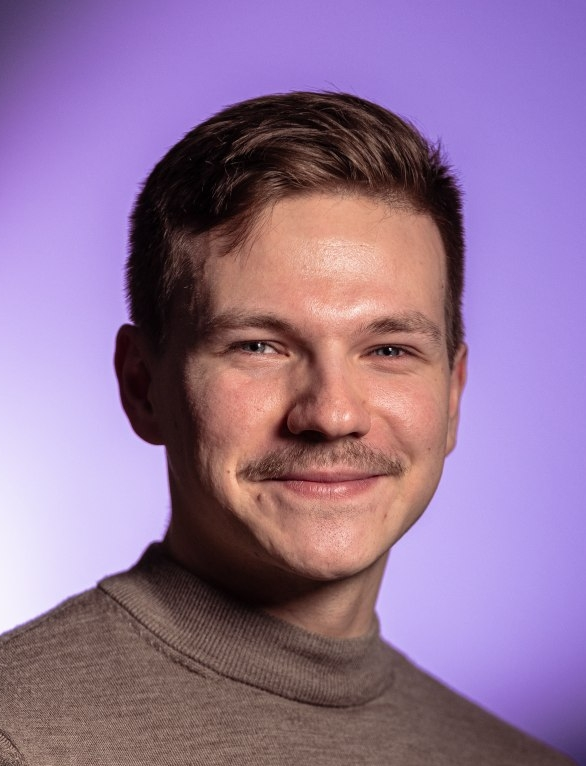
\includegraphics[height=40mm,trim={0cm 0 0cm 0},clip]{cvpic.jpg}}
    {
    % name
    \cvname{Jussi Hietanen}

    % address
    \cvpersonalinfolinewithicon{height=4mm}{072-location.pdf}{
        Espoo, Finland
    }

    % phone number
    \cvpersonalinfolinewithicon{height=4mm}{067-phone.pdf}{
        +358 50\,911\,5671
    }

    % email address
    \cvpersonalinfolinewithicon{height=4mm}{070-envelop.pdf}{
        \href{mailto:jussi.hietanen@iki.fi}{jussi.hietanen@iki.fi}
    }

    % LinkedIn account
    \cvpersonalinfolinewithicon{height=4mm}{458-linkedin.pdf}{
        \href{https://www.linkedin.com/in/jussi-hietanen-ba0320107/}{jussi-hietanen-ba0320107}
    }
    
    \cvpersonalinfolinewithicon{height=4mm}{GitHub-Mark-120px-plus.png}{
        \href{https://github.com/jussihi}{jussihi}
    }

    % date of birth
    % not here :-)
}

\vspace{2em}


% work experience
% ---------------

\cvsection{LATEST WORK EXPERIENCE}

\cvitem{
    \cvdurationstyle{March  2021 -- June 2022}
}{
    \cvtitle{Security Engineer}

    Tuxera Oy, Espoo

    \begin{itemize}[leftmargin=*]
        \item Created tools to automatically discover vulnerabilities in file system drivers (C, C++, Python)
        \item Security incident \& vulnerability management
    \end{itemize}
}


\cvitem{
    \cvdurationstyle{January  2019 -- March 2021}
}{
    \cvtitle{Research assistant}

    Aalto University, Espoo

    \begin{itemize}[leftmargin=*]
        \item Implementation of a safe GNU+Linux operating system to create a controllable electronic examination environment with tools written in C \& C++
    \end{itemize}
}


\cvitem{
    \cvdurationstyle{September  2018 -- December 2018}
}{
    \cvtitle{Junior Engineer in Test}

    Tuxera Oy, Espoo

    \begin{itemize}[leftmargin=*]
        \item Testing of Tuxera's filesystem kernel drivers \& integration of new hardware for testing
    \end{itemize}
}


\cvitem{
    \cvdurationstyle{June 2017 -- September 2017}
}{
    \cvtitle{Research assistant, Bachelor's thesis worker}

    Aalto University, Espoo

    \begin{itemize}[leftmargin=*]
        \item C++ implementation of the PDCP protocol layer in NB-IoT research team
    \end{itemize}
}

\cvitem{
    \cvdurationstyle{January 2017 -- December 2018}
}{
    \cvtitle{Teaching assistant on different university courses}

    Aalto University, Espoo

    \begin{itemize}[leftmargin=*]
        \item Teaching the basics of C programming, Computer Networks and C++ both in teaching assistant and head assistant roles
    \end{itemize}
}


\cvitem{
    \cvdurationstyle{Before 2017}
}{
    \cvtitle{Different temporary jobs}

    \begin{itemize}[leftmargin=*]
        \item Spring/Summer of 2015/2016 -- Atria Oyj, Seinäjoki -- Seasonal worker at Atria Oyj as a meat packer
        \item Fall 2014 -- Finnish Defence Forces, Riihimäki -- Contract soldier as 2nd lieutenant.
        \item Spring 2013 -- Different schools, Seinäjoki area -- Substitute teacher in elementary and secondary schools
    \end{itemize}
}


% education
% ---------

\cvsection{EDUCATION}


% bachelor's
\cvitem{
    \cvdurationstyle{2015 -- 2018}
}{
    \cvtitle{Bachelors's degree in Information Technology}

    School of Electrical Engineering, Aalto University

    \begin{itemize}[leftmargin=*]
        \item Courses regarding digital signal processing, programming (mainly C, python \& C++), and mathematical subjects.
    \end{itemize}
}

% master's
\cvitem{
    \cvdurationstyle{2018 -- 2021}
}{
    \cvtitle{Master's degree in Computer Science}

    School of Science, Aalto University

    \begin{itemize}[leftmargin=*]
        \item Major in Security and Cloud Computing, which was very security-oriented.
        \item Master's thesis about the system security (threat modeling and analysis) of the customized electronic exam environment described above.
    \end{itemize}
}


\newpage

\vspace*{2em}

% skills
% ------

\cvsection{SKILLS}

\vspace{\cvbetweensectionandheadingextraskipamount}

% Languages
\cvitem{
    \cvheadingstyle{Languages}
}{
    Finnish -- native

    English -- fluent
}

% Programming languages
\cvitem{
    \cvheadingstyle{Programming / scripting}
}{
    Most experienced with C, C++, Python, \& Unix shell scripting
    \begin{itemize}
        \item Very familiar with basic \& advanced C/C++ programming (\& boost library).
        \item Familiar with POSIX interfaces and Windows/Linux kernel driver development.
        \item Familiar with EDK 2, see the SMM rootkit from my GitHub.
        \item Fast learner when working with new project or library code bases!
    \end{itemize}
    
	\vspace{0.2cm}
    Familiar with C\#, MatLab, MySQL, HTML, CSS, legacy PHP, legacy x86 asm...
    \begin{itemize}
        \item I have used programming languages listed above in various personal projects.
    \end{itemize}
    
}

% Skills
\cvitem{
    \cvheadingstyle{Other skills}
}{
    
    -- Generally experienced GNU/Linux user

    -- Good understanding of computer networks
    
    -- Containers (docker)
    
    -- CI/CD (personal experience with GitLab's and GithUb's CI/CD pipelines)
    
    -- Familiar with software project management methodologies (Agile, waterfall etc.)
    
    -- I get along well with people, and I am not afraid to perform or teach in front of a larger crowd

}


% additional info
% ---------------

\cvsection{PERSONAL INTERESTS}

\vspace{\cvbetweensectionandheadingextraskipamount}


\cvitem{
    \cvheadingstyle{Chess and board games}
}{
    -- I play online chess almost daily

    -- I have programmed a simple chess AI, also implemented a novel AI for "BattleSheep" board game
    
}


\cvitem{
    \cvheadingstyle{Linux on smartphones}
}{

    -- PinePhone Braveheart owner
    
    -- Also running SailfishOS on my daily driver to make my life harder
    
    -- Waiting for and maybe unknowingly living the first years of proper Linux on phones (since I had my first MeeGo phone in 2012)
    
}


\cvitem{
    \cvheadingstyle{Hi-Fi}
}{
    -- I enjoy listening to good quality music through a good quality audio setup
}


\cvitem{
    \cvheadingstyle{Physical hobbies}
}{
    -- Hiking, gym, jogging, practical shooting
}

\end{document}
